
\begin{frame}
\frametitle{Reglas básicas}
\begin{itemize}
\item Se recomienda puntualidad y asistencia a las sesiones.
\item Respecto hacia el profesor y hacia sus compañeros y compañeras.  
\item No se permite el ingreso y/o ingestión de \textbf{Alimentos} ni \textbf{Bebidas} de ningún tipo a la clase. 
\item Solo se puede usar \textbf{AUDIFONOS O DISPOSITIVOS MANO-LIBRES EN CLASE} previa autorización por parte del profesor. Cualquier uso no AUTORIZADO es motivo de amonestación  al estudiante, y expulsión en caso de reincidir sin derecho a r\'eplica. 
\end{itemize}
\end{frame}

\begin{frame}
\frametitle{Uso del Teléfono Inteligente}
\begin{itemize}
\item Se recomienda no utilizarlo durante el transcurso de la clase. Depende del comportamiento del grupo que esto no sea aplicado...
\begin{block}{Resguardo del teléfono inteligente}
De ser necesario, se solicitará al INICIO de la CLASE a todos los asistentes a la clase (incluyendo al profesor) guardar su telefono en una caja, la cual será cerrada, regresando su telefono al finalizar la SESION.
\begin{center}
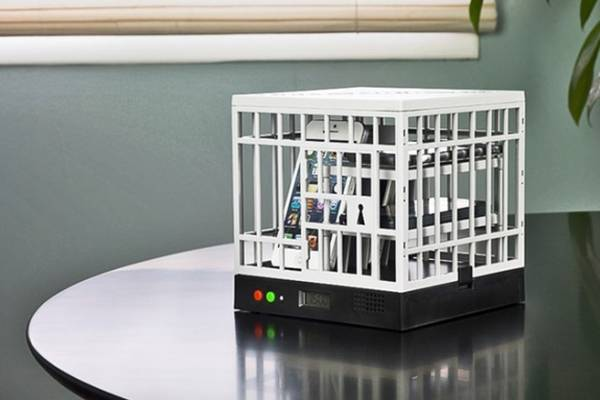
\includegraphics[width=0.35\linewidth]{ReglasBasicas/CajaFuerteCeluar.jpg}
\end{center}
\end{block}
\end{itemize}
\end{frame}



\begin{frame}
\frametitle{Pase de Lista}
\begin{itemize}
\item Se pasa lista al inicio de la clase. En caso de reincorporaci\'on tard\'ia, se pone un retardo.
\item DOS RETARDOS equivalen a una INASISTENCIA, que no es JUSTIFICABLE.
\item Para justificar una inasistencia, es necesario cumplir con los siguientes pasos:
\begin{itemize}	 
\item Agendar una asesoría de la clase mediante el SIITA. Una vez hecho esto, solicitar al profesor confirmación para actualizar su registro de inasistencia de tal dia en la lista de asistencia de la clase.
\item En el TEMA de la ASESORIA debe poner \textbf{``JUSTIFICACION DE INASISTENCIA DEL DIA X/YY/ZZZZ''}. De no hacer lo anterior, no será considerada dicha justificación. 
\item \textbf{DEBEN agendar una asesoria por cada fecha de INASISTENCIA (5 faltas, 5 asesorias). }
\item \textbf{NO ES NECESARIO ENVIAR correo electrónico al profesor -- }
\end{itemize}
\end{itemize}
\end{frame}


\begin{frame}
\frametitle{Alumnos con Empleo (1)}
\begin{itemize}
\item Al NO alcanzar un 80\% de asistencia, el estudiante pierde su derecho de ser EVALUADO
\end{itemize}
\begin{block}{Alumnos VIPs}
En caso de tener un empleo formal dentro o fuera de la ciudad, es necesario entregar una \textbf{constancia laboral} que acredite el horario que se esta cubriendo (en el caso de locales, este horario se debe empalmar con el de la materia). En esa constancia debe acreditar que se esta haciendo labores de manera presencial en tal ubicacion. Esto lo dispensa solo del requisito de las asistencias, mas no de los proyectos que deban entregarse. Incluso pudiera solicitarle presentar avance de manera ``remota'' durante alguna de las clases. Enviar esa constancia con copia para el director de carrera.
\end{block}
\end{frame}


\begin{frame}
\frametitle{Alumnos con Empleo (2)}
\begin{itemize}
\item La justificacion de inasistencias por \textit{actividad laboral} se considerar\'a a partir del momento de la recepci\'on de dicha constancia en el correo del instructor (y no a partir de la fecha indicada en la constancia), por lo que si se recibe de manera tardia (con mas de una semana de retardo), dichas inasistencias NO SERAN justificadas.
\item La justificación será válida si el estudiante programa \textbf{POR LO MENOS} dos asesorías por semana. De no hacerlo, pierde el beneficio de la justificación y se aplican las reglas anteriormente establecidas. 
\end{itemize}

\end{frame}






